% mnras_template.tex 
%
% LaTeX template for creating an MNRAS paper
%
% v3.0 released 14 May 2015
% (version numbers match those of mnras.cls)
%
% Copyright (C) Royal Astronomical Society 2015
% Authors:
% Keith T. Smith (Royal Astronomical Society)

% Change log
%
% v3.0 May 2015
%    Renamed to match the new package name
%    Version number matches mnras.cls
%    A few minor tweaks to wording
% v1.0 September 2013
%    Beta testing only - never publicly released
%    First version: a simple (ish) template for creating an MNRAS paper

%%%%%%%%%%%%%%%%%%%%%%%%%%%%%%%%%%%%%%%%%%%%%%%%%%
% Basic setup. Most papers should leave these options alone.
\documentclass[fleqn,usenatbib]{mnras}

% MNRAS is set in Times font. If you don't have this installed (most LaTeX
% installations will be fine) or prefer the old Computer Modern fonts, comment
% out the following line
\usepackage{newtxtext,newtxmath}
% Depending on your LaTeX fonts installation, you might get better results with one of these:
%\usepackage{mathptmx}
%\usepackage{txfonts}

% Use vector fonts, so it zooms properly in on-screen viewing software
% Don't change these lines unless you know what you are doing
\usepackage[T1]{fontenc}
\usepackage{ae,aecompl}


%%%%% AUTHORS - PLACE YOUR OWN PACKAGES HERE %%%%%

% Only include extra packages if you really need them. Common packages are:
\usepackage{graphicx}	% Including figure files
\usepackage{amsmath}	% Advanced maths commands
\usepackage{amssymb}	% Extra maths symbols

%%%%%%%%%%%%%%%%%%%%%%%%%%%%%%%%%%%%%%%%%%%%%%%%%%

%%%%% AUTHORS - PLACE YOUR OWN COMMANDS HERE %%%%%

% Please keep new commands to a minimum, and use \newcommand not \def to avoid
% overwriting existing commands. Example:
%\newcommand{\pcm}{\,cm$^{-2}$}	% per cm-squared

%%%%%%%%%%%%%%%%%%%%%%%%%%%%%%%%%%%%%%%%%%%%%%%%%%

%%%%%%%%%%%%%%%%%%% TITLE PAGE %%%%%%%%%%%%%%%%%%%

% Title of the paper, and the short title which is used in the headers.
% Keep the title short and informative.
\title[GPM for Faraday Depth Spectra]{Gaussian Process Modeling to Recover Faraday Depth Spectra}

% The list of authors, and the short list which is used in the headers.
% If you need two or more lines of authors, add an extra line using \newauthor
\author[S.~W.~Ndiritu et al.]{
S.~W.~Ndiritu,$^{1}$\thanks{E-mail: simon.ndiritu@postgrad.manchester.ac.uk
 (SWN)}
A.~M.~M.~Scaife$^{1}$,
A.~N.~Other$^{1}$...
\\
% List of institutions
$^{1}$ Jodrell Bank Centre for Astrophysics, School of Physics and Astronomy, University of Manchester, Alan Turing Building,\\ Oxford Road, Manchester, M13 9PL, UK
}

% These dates will be filled out by the publisher
\date{Accepted XXX. Received YYY; in original form ZZZ}

% Enter the current year, for the copyright statements etc.
\pubyear{2015}

% Don't change these lines
\begin{document}
\label{firstpage}
\pagerange{\pageref{firstpage}--\pageref{lastpage}}
\maketitle

% Abstract of the paper
\begin{abstract}
This is a simple template for authors to write new MNRAS papers.
The abstract should briefly describe the aims, methods, and main results of the paper.
It should be a single paragraph not more than 250 words (200 words for Letters).
No references should appear in the abstract.
\end{abstract}

% Select between one and six entries from the list of approved keywords.
% Don't make up new ones.
\begin{keywords}
keyword1 -- keyword2 -- keyword3
\end{keywords}

%%%%%%%%%%%%%%%%%%%%%%%%%%%%%%%%%%%%%%%%%%%%%%%%%%

%%%%%%%%%%%%%%%%% BODY OF PAPER %%%%%%%%%%%%%%%%%%

\section{Introduction}

Polarisation measurements from radio telescopes with broadband receiver systems have changed the way in which we investigate magnetised astrophysical plasmas by enabling the use of the RM synthesis method (Burn 1966; Brentjens \& de~Bruyn 2005). In this method the Fourier relationship between polarized intensity as a function of wavelength-squared and the Faraday dispersion function is exploited to recover the polarized intensity as a function of Faraday depth, $\phi$, such that
%
\begin{equation}
\label{eq:fourier}
F(\phi) = \int_{-\infty}^{\infty}{ P(\lambda^2){\rm e}^{-2i\phi \lambda^2}~{\rm d}\lambda^2 },
\end{equation}
%
where 
%
\begin{equation}
P(\lambda^2) = |P(\lambda^2)|{\rm e}^{2i\chi(\lambda^2)} = Q(\lambda^2) + iU(\lambda^2).
\end{equation}

Although conceptually simple, in practical terms the implementation of this method and the interpretation of the resulting Faraday dispersion function are complicated by a number of factors. The first of these complications is that the Stokes pseudo-vectors $Q$ and $U$ are not sampled natively in wavelength-squared but linearly in frequency. A further complication is that Eq.~\ref{eq:fourier} does not represent a true Fourier relationship as $P(\lambda^2)$ does not exist at $\lambda^2 < 0$. Since $F(\phi)$ is not necessarily a purely real quantity this represents a fundamental limitation in attempting to reconstruct an unknown Faraday dispersion function from measured values of $P(\lambda^2)$. An additional limitation comes from the finite bandwidth and hence range of wavelength-squared, $\Delta (\lambda^2)$, measured by a radio telescope receiver, as well as the potentially incomplete sampling over this bandwidth due to various effects (RFI, instrumental problems etc.) that require flagging (excision) of specific frequency channel data during an observation.

In order to exploit the use of Fast Fourier Transforms (FFTs), computational approaches to RM Synthesis employ an initial processing step to re-bin spectral data, $Q(\nu)~\&~U(\nu)$, into regularly spaced arrays of $\lambda^2$. This approach produces regularly sampled data arrays, $Q(\lambda^2)~\&~U(\lambda^2)$ that are multiplied by a weighting function, $W(\lambda^2)$, which is non-zero where measurements are present but which will also contain a (potentially significant) number of zero-valued elements due to the non-linear mapping of $\nu$ to $\lambda^2$. This  multiplication results in the convolution of the Faraday dispersion function with a transfer function,
%
\begin{equation}
{\rm RMTF}(\phi) = \frac{\int_{-\infty}^{\infty} { W(\lambda^2){\rm e}^{-2i\phi\lambda^2}~{\rm d}\lambda^2 }}{\int_{-\infty}^{\infty} { W(\lambda^2)~{\rm d}\lambda^2 }},
\end{equation}
%
known as the \emph{rotation measure transfer function}, RTMF$(\phi)$. Consequently, the complications caused by both the $\lambda^2 < 0$ problem and the mapping of linear frequency to wavelength-squared may be encapsulated in the weighting function $W(\lambda^2)$ and its Fourier counterpart, RMTF($\phi$). Although attempts have been made to deconvolve the RMTF from the Faraday depth spectra (e.g. Heald et al. ???) the  methods are inherently underconstrained due to the $P(\lambda^2<0) = \varnothing$ problem, resulting in a statistical ambiguity in the results.

In this work we explore the potential for replacing both the re-binning processing step and the consequent deconvolution in Faraday depth necessitated by the RMTF with a Gaussian Process Modelling (GPM) approach. The contents of this paper are as follows, in \S~\ref{sec:method} we describe the underlying GPM methodology including a description of the covariance kernel functions employed and the optimization of their hyper-parameters; in \S~\ref{sec:sims} we illustrate the use of the method on simulated data and in \S~\ref{sec:realdata} we demonstrate the method using real data from the MeerKAT telescope; in \S~\ref{sec:disc} we discuss the implications of these results and compare the outputs to those using a more traditional RM Synthesis approach. 

\section{GPM in Astronomy}
\label{sec:astrogpm}

\textcolor{green}{This section needs rewording - just copied and pasted from previous papers at the moment.}

Gaussian Process Modelling (GPM) has been used widely in astronomy, for example in cosmic microwave background estimation (Bond \& Efstathiou 1987; Bond et al. 1999; Wandelt \& Hansen 2003), modelling correlated instrumental noise (Gibson et al. 2012), and for spectroscopic calibration (Evans et al. 2015; Czekala et al. 2017).

More recently, GPs have been used in the stellar and exoplanet fields within astronomy to capture stellar variability or instrumental systematics (see e.g. Gibson et al. 2012; Dawson et al. 2014; Haywood et al. 2014; Barclay et al. 2015; Czekala et al. 2015; Evans et al. 2015; Haywood 2015; Rajpaul et al. 2015; Vanderburg et al. 2015; Aigrain, Parviainen \& Pope 2016; Rajpaul, Aigrain & Roberts 2016; Littlefair et al. 2017). They are useful in regression problems involving any stochastic process, specifically when the probability distribution for the process is a multivariate Gaussian.

The application of GPM to time series modelling can be extended to the {\it frequency series modelling} required for studies of Faraday depth spectra in cosmic magnetisn science...

\section{Method}
\label{sec:method}

The basic premise of GPM is that, instead of employing a physically motivated or semi-empirical parametric model to describe a dataset, we can instead assume that the data, $y(x)$, represent the realization of a random Gaussian process,
%
\begin{equation}
y(x) = N(\mu(x), K(x,x)),
\end{equation}
%
where $K(x,x)$ is the matrix that defines the degree of covariance between every pair of measurement positions, $(x,x')$, and $\mu(x)$ is an underlying mean function, which in this case is considered to be zero-valued. In the case of non-negligible polarization leakage, this would manifest as $\mu(x)\neq 0$.

The expected value of the data at all other positions, $x_{\ast}$, can be calculated as a posterior mean, $mu_{\ast}$, with an associated posterior variance, $C_{\ast}$, such that
%
\begin{eqnarray}
\label{eq:postmu} \mu_{\ast} &=&  K(x_{\ast},x)^T K(x,x)^{-1} y  \\
\label{eq:postcov} C_{\ast} &=&  K(x_{\ast},x_{\ast}) - K(x_{\ast},x)^T K(x,x)^{-1} K(x_{\ast},x) 
\end{eqnarray}
%
(see e.g. Rasmussen \& Williams; Roberts et~al. 2012).

For polarization data measured at regular intervals in frequency (spectral channels) and hence irregular intervals in $\lambda^2$, the posterior mean can be used to predict the values of the polarization data at regular intervals, $\lambda_{\ast}^2$, avoiding the need for explicit re-binning of the data, and the posterior variance can be used to define the weighting function $W(\lambda_{\ast}^2)$ at those positions and hence calculate the RMTF. 

\subsection{Kernel Definition}
\label{sec:kernels} 

The covariance matrix used in Eqs.~\ref{eq:postmu}~\&~\ref{eq:postcov} can be populated analytically using a kernel function, $k$, that defines the degree of covariance for each measurement separation,

\begin{equation}
K(x,x) = \left(
\begin{array}{cccc}
k(x_1,x_1) & k(x_1,x_2) & ... & k(x_1,x_n) \\
k(x_2,x_1) & k(x_2,x_2) & ... & k(x_2,x_n) \\
\vdots & \vdots & \vdots & \vdots \\
k(x_n,x_1) & k(x_n,x_2) & ... & k(x_n,x_n) 
\end{array}
\right),
\end{equation}
%
where $k(x_1,x_2)$ is the covariance between two measurements at a separation $|x_1 - x_2|$.

For complex-valued polarization measurements, each element $k_{ij} = k(x_i, x_j)$ is a $2 \times 2$ matrix, where
%
\begin{equation}
k_{ij} = k(x_i, x_j) = \begin{bmatrix} k_{\rm QQ}(x_i,x_j) & k_{\rm QU}(x_i,x_j) \\ k_{\rm UQ}(x_i,x_j) & k_{\rm UU}(x_i,x_j) \end{bmatrix}.
\end{equation}
%


\subsection{Covariance kernel definition}
\label{sec:kernels}

For the application to radio polarization data we use a compound covariance kernel. The contributions to this kernel comprise covariance arising both from the expected signal and from the properties of the measurement data. 

Faraday rotation results in periodicity in $Q(\lambda^2)$ and $U(\lambda^2)$. We model this using an exponential sine-squared kernel,
%
\begin{equation}
\label{eq:expsinsq}
k_1(x_i,x_j)=h_1 \exp \left( \Gamma \sin^2 \left[ \frac{\pi}{P}|x_i - x_j|\right] \right).
\end{equation}
%
However, in order to allow local deviations from exact periodicity we modulate this kernel with the exponential-squared kernel,
%
\begin{equation}
\label{eq:expsq}
k_2(x_i,x_j)=h_2 \exp \left( \frac{ -(x_i - x_j)^2}{2\sigma^2} \right),
\end{equation}
%
such that the combined kernel becomes
%
\begin{equation}
\label{eq:combkernel}
k_1 k_2 =h \exp \left( - \frac{(x_i - x_j)^2}{2 \sigma^2} \right) \exp \left( \Gamma \sin^2 \left[ \frac{\pi}{P}|x_i - x_j|\right] \right),
\end{equation}
%
where $h = h_1 h_2$

To these signal contributions we also add a white noise kernel to account for independent measurement noise,
%
\begin{equation}
\label{eq:noisekernel}
k_3(x_i,x_j)= h_3 \delta_{ij}
\end{equation}
%
Consequently, the complete covariance kernel is given by
%
\begin{equation}
k(x_i,x_j) = k_1 k_2 + k_3,
\end{equation}
%
where the contributions of the various component kernels are governed by the values of their hyper-parameters.

\subsection{Hyper-parameter Estimation}
\label{sec:parms}

The values of the hyper-parameters can be optimized by evaluation of a likelihood function using the measured data. Polarization data are complex valued, 
%
\begin{equation}
P(\nu) = Q(\nu) + iU(\nu)
\end{equation}
%
and so the loglikelihood function can be broken down,
%
\begin{equation}
\log L_{\rm P} = \log L_{\rm Q} + \log L_{\rm U}
\end{equation}
%
The components of this likelihood are
%
\begin{eqnarray}
\log L_{\rm Q} &=& -\frac{1}{2}(Q - \mu_{\rm Q})^{\rm T}K_{\rm Q}^{-1}(Q - \mu_{\rm Q}) - \frac{1}{2}\ln |K_{\rm Q}|\\
\log L_{\rm U} &=& -\frac{1}{2}(U - \mu_{\rm U})^{\rm T}K_{\rm U}^{-1}(U - \mu_{\rm U}) - \frac{1}{2}\ln |K_{\rm U}|
\end{eqnarray}
%
where,
%
\begin{eqnarray}
\mu_{Q} &=& K_{\rm Q}(x_{\ast},x)^T K_{\rm Q}(x,x)^{-1} Q\\
\mu_{U} &=& K_{\rm U}(x_{\ast},x)^T K_{\rm U}(x,x)^{-1} U. 
\end{eqnarray}
%


\subsection{Re-sampling Definition}
\label{sec:resamp}

There are two aspects that can be addressed through resampling. The first is the regularity of measurements in $\lambda^2$-space. This regularity reduces the effect of the transfer function in Faraday depth and lowers the contamination from the RMTF side-lobes. The second effect is to increase the accessible range of $\lambda^2$-space. This can be achieved by extending the maximum and minimum limits in $\lambda^2$-space. 

To re-sample onto a regular grid in $\lambda^2$-space we need to set a step size $(\delta \lambda_{\ast}^2)$ as our regular interval. The step size that we choose will determine the maximum Faraday depth to which we have sensitivity. We can therefore chose a step size based on our desired range of Faraday depths. In practice the data will normally allow for higher maximum values than are required as astrophysical Faraday depths are typically small due to the correspondingly low electron densities and magnetic field strengths, even in the presence of very large path lengths. For Galactic fields, Faraday depths are normally limited to a range of $\pm10$\,rad\,m$^{-2}$, for external galaxies they are in the range $\sim100$\,rad\,m$^{-2}$ and for galaxy clusters typically $<1000$\,rad\,m$^{-2}$. With the exception of a few rare cases, there is no need to sample $\lambda^2$ more finely than corresponds to these values, such that,
%
\begin{equation}
 \delta (\lambda^2) = \frac{\sqrt{3}}{||\phi_{\rm max}||}.
\end{equation}
%
In what follows we specify a maximum Faraday depth of 200\,rad\,m$^{-2}$.

To extend the bandwidth $\Delta \lambda^2$, we apply the same approach and discard the five largest separations in the measured data. We then adopt the sixth largest separation as an extension in $\lambda^2$-space. This is represented graphically in Figure~\ref{fig:resampling}. The effect of this increase in available $\Delta \lambda^2$ is to improve the resolution somewhat in Faraday depth space,
%
\begin{equation}
\delta \phi = \frac{2\sqrt{3}}{\Delta (\lambda^2)},
\end{equation}
%
and to increase the sensitivity to extended Faraday structures,
%
\begin{equation}
\Delta \phi = \frac{\pi}{\lambda_{\rm min}^2}.
\end{equation}

\begin{figure}
\caption{\label{fig:resampling}}
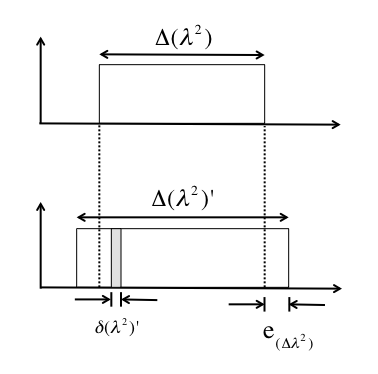
\includegraphics[width=0.5\textwidth]{./FIGURES/faraday_resampling.png}
\end{figure}

\section{Application to Simulated Data}
\label{sec:sims}

We demonstrate the use of the method on two examples: (1) a simple Faraday Thin scenario, and (2) a more complex scenario involving both Faraday Thin and Faraday Thick components. This second scenario corresponds to the example geometry outlined in \S~1 of Brentjens \& de~Bruyn (2005).

\vskip .1in
\noindent
\textbf{Scenario One} In this scenario we assume  polarized emission from the lobe of a radio galaxy has a single valued Faraday depth of 10\,rad\,m$^{-2}$ such that,
%
\begin{equation}
F_{\rm rg}(\phi) = 0.25\delta(\phi - \phi_1),
\end{equation}
%
where $\phi_1 = 10$\,rad\,m$^{-2}$ and consequently the measured polarization as a function of wavelength-squared will be:
%
\begin{eqnarray}
P_{\rm rg}(\lambda^2) &=& 0.25 \exp (2i\phi_1 \lambda^2) \\
&=& 0.25 \cos (2\phi_1 \lambda^2) + 0.25 i \sin (2\phi_1 \lambda^2).
\end{eqnarray}

We assume that this signal is measured over a bandwidth of ?? with channels at regularly spaced frequency intervals of width ??. We map each channel frequency to a corresponding value of $\lambda^2$. For each measurement we assume that $(Q, U, \sigma_{\rm Q}, \sigma_{\rm U})$ are recorded, where $Q$ corresponds to the real part of the polarization and $U$ corresponds to the imaginary component. 

\vskip .1in
\noindent
\textbf{Scenario Two} In this scenario we adopt the line of sight geometry of Brentjens \& de~Bruyn (2005). 

\begin{equation}
F_{\rm gal}(\phi) = \begin{cases}
(2\phi_{\rm fg})^{-1} & -\phi_{\rm fg}~<~\phi~<~\phi_{\rm fg} \\
0 & {\rm elsewhere}
\end{cases} 
\end{equation}

\begin{equation}
P_{\rm gal}(\lambda^2) = \frac{\sin (2\phi_{\rm fg} \lambda^2)}{2\phi_{\rm fg}\lambda^2}
\end{equation}
%
and the total polarization is given by
%
\begin{equation}
P_{\rm tot}(\lambda^2) = P_{\rm gal}(\lambda^2) + P_{\rm rg}(\lambda^2)
\end{equation}

\subsection{Faraday Depth Spectra}

\subsection{Parameter Estimation}

To optimize the hyper-parameters we use MCMC to explore the posterior probability distribution. We use 500 samples for the burn-in then take the maximum likelihood hyper-parameter values from the burn-in and perturb them by adding noise at a level of $10^{-5}$. We then use these perturbed values to start a production run of 5000 samples.

\subsubsection{Fast Kernel Estimation using C{\'e}l{\'e}rit{\'e}}

The {\tt celerite} Gaussian processing library [REF] implements a fast separable covariance kernel that can be evaluated for $n$ data points with a linear complexity of $\mathcal{O}(n)$. The kernel has a generalised form, 
%
\begin{equation}
    k(x_1,x_2) = \sum_{i=1}^{J}{\alpha_i {\rm e}^{-\beta_i |x_1 - x_2|} + \alpha_i^{\ast} {\rm e}^{-\beta_i^{\ast} |x_1 - x_2|}},
\end{equation}
%
which can be used to produce an approximation to the quasi-periodic kernel given in Eq.~\ref{eq:combkernel} with the form, 
%
\begin{equation}
k(x_1,x_2)=h\,{\rm e}^{-c|x_1 - x_2|}\left[\cos\left(\frac{2\pi|x_1 - x_2|}{P}\right)\right],
\end{equation}
%
where $h$, $c$ and $P$ are hyper-parameters.


\section{Application to Real Data}
\label{sec:realdata}

\section{Discussion}
\label{sec:disc}

\subsection{Kernel selection}

For each model we find the maximum likelihood using L-BFGS-B optimisation and use this value to compute the Bayesian Information Criteria (BIC; Schwarz et al. 1978),
%
\begin{equation}
{\rm BIC} = -2 \log L^\ast + K \log N,
\end{equation}
%
the Akaike Information Criterion (AIC; Akaike 1974),
%
\begin{equation}
{\rm AIC} = 2 K - 2\log L^\ast,
\end{equation}
%
and the corrected AIC (AICc; Hurvich \& Tsai 1989),
%
\begin{equation}
{\rm AICc} = {\rm AIC} + \frac{2K(K+1)}{N - K - 1},
\end{equation}
%
where $L^\ast$ is the maximum value of the likelihood, $K$ is the number of free parameters, and $N$ is the number of data points. 

These information criteria are designed to evaluate the amount of information lost by a particular model. The model that loses the least information (i.e. has the lowest valued information criterion) is considered to be the preferred model. 

The BIC is considered to be a powerful model selection tool when the `true' model is in the set of test models. For simulated data such as that used here, this is considered appropriate; however, in the case of true empirical data the AIC is considered to be a more appropriate criterion. Furthermore, the {\it corrected} AIC places a stronger complexity penalty on models used with finite data series than the original AIC. In the case of small sample sizes it is considered to be more appropriate and accurate for finding the preferred model. For a more detailed comparison of the different information criteria we refer the reader to Burnham \& Anderson (2002) or XXX. 

\begin{table}
    \centering
    \begin{tabular}{l|cc|ccc}
    \hline
    Model & N & K & BIC & AIC & AICc \\\hline
     k_1 + k_3               & & 4 & & & \\
     k_2 + k_3               & & 3 & & & \\
     k_1k_2 + k_3            & & 5 & & & \\
     k_1k_2 + k_1'k_2' + k_3 & & 9 & & & \\\hline 
    \end{tabular}
    \caption{Model comparison for Scenario One (simple) Faraday depth spectrum.}
    \label{tab:infocriteria}
\end{table}

\begin{table}
    \centering
    \begin{tabular}{l|cc|ccc}
    \hline
    Model & N & K & BIC & AIC & AICc \\\hline
     k_1 + k_3               & & 4 & & & \\
     k_2 + k_3               & & 3 & & & \\
     k_1k_2 + k_3            & & 5 & & & \\
     k_1k_2 + k_1'k_2' + k_3 & & 9 & & & \\\hline 
    \end{tabular}
    \caption{Model comparison for Scenario Two (complex) Faraday depth spectrum.}
    \label{tab:infocriteria}
\end{table}

\subsection{Computational considerations}

The computational complexity of $\lambda^2$-gridding is $\mathcal{O}(n^2)$ and the FFT for RM Synthesis scales as $\mathcal{O}(m\log m)$, where $n$ is the number of input frequency channels and $m$ is the number of regular intervals in the $\lambda^2$ grid. For typical applications, $m>n$. 

Whilst the complexity for evaluating the likelihood of a Gaussian process using a standard approach is known to scale as $\mathcal{O}(m^3)$, the separable approach used by the {\tt celerite} library scales linearly as $\mathcal{O}(m)$. Since one might assume that the 


\section{Conclusions}


\section*{Acknowledgements}

The Acknowledgements section is not numbered. Here you can thank helpful
colleagues, acknowledge funding agencies, telescopes and facilities used etc.
Try to keep it short.

%%%%%%%%%%%%%%%%%%%%%%%%%%%%%%%%%%%%%%%%%%%%%%%%%%

%%%%%%%%%%%%%%%%%%%% REFERENCES %%%%%%%%%%%%%%%%%%

% The best way to enter references is to use BibTeX:

%\bibliographystyle{mnras}
%\bibliography{example} % if your bibtex file is called example.bib


% Alternatively you could enter them by hand, like this:
% This method is tedious and prone to error if you have lots of references
\begin{thebibliography}{99}
\bibitem[\protect\citeauthoryear{Author}{2012}]{Author2012}
Author A.~N., 2013, Journal of Improbable Astronomy, 1, 1
\bibitem[\protect\citeauthoryear{Others}{2013}]{Others2013}
Others S., 2012, Journal of Interesting Stuff, 17, 198
\end{thebibliography}

%%%%%%%%%%%%%%%%%%%%%%%%%%%%%%%%%%%%%%%%%%%%%%%%%%

%%%%%%%%%%%%%%%%% APPENDICES %%%%%%%%%%%%%%%%%%%%%

\appendix

\section{Some extra material}

If you want to present additional material which would interrupt the flow of the main paper,
it can be placed in an Appendix which appears after the list of references.

%%%%%%%%%%%%%%%%%%%%%%%%%%%%%%%%%%%%%%%%%%%%%%%%%%


% Don't change these lines
\bsp	% typesetting comment
\label{lastpage}
\end{document}

% End of mnras_template.tex